%===============================================================================
% LaTeX sjabloon voor de bachelorproef toegepaste informatica aan HOGENT
% Meer info op https://github.com/HoGentTIN/latex-hogent-report
%===============================================================================

\documentclass[dutch,dit,thesis]{hogentreport}

% TODO:
% - If necessary, replace the option `dit`' with your own department!
%   Valid entries are dbo, dbt, dgz, dit, dlo, dog, dsa, soa
% - If you write your thesis in English (remark: only possible after getting
%   explicit approval!), remove the option "dutch," or replace with "english".

\usepackage{lipsum} % For blind text, can be removed after adding actual content
\usepackage{glossaries}

%% Pictures to include in the text can be put in the graphics/ folder
\graphicspath{{graphics/}}
\makeglossaries


%%---------- Document metadata -------------------------------------------------
\author{Laurent Duquesnoy}
\supervisor{Dhr. J. Claes}
\cosupervisor{Mr. S. Dewolf}
\title%
    {Optimalisatie van de administratieve workflow in juridische kantoren: automatisering van repetitieve taken}
\academicyear{\advance\year by -1 \the\year--\advance\year by 1 \the\year}
\examperiod{1}
\degreesought{\IfLanguageName{dutch}{Professionele bachelor in de toegepaste informatica}{Bachelor of applied computer science}}
\partialthesis{false} %% To display 'in partial fulfilment'
%\institution{Internshipcompany BVBA.}

%% Add global exceptions to the hyphenation here
\hyphenation{back-slash}

%% The bibliography (style and settings are  found in hogentthesis.cls)
\addbibresource{bachproef.bib}            %% Bibliography file
\addbibresource{../voorstel/voorstel.bib} %% Bibliography research proposal
\defbibheading{bibempty}{}

%% Prevent empty pages for right-handed chapter starts in twoside mode
\renewcommand{\cleardoublepage}{\clearpage}

\renewcommand{\arraystretch}{1.2}

%% Content starts here.
\begin{document}

%---------- Front matter -------------------------------------------------------

\frontmatter

\hypersetup{pageanchor=false} %% Disable page numbering references
%% Render a Dutch outer title page if the main language is English
\IfLanguageName{english}{%
	%% If necessary, information can be changed here
	\degreesought{Professionele Bachelor toegepaste informatica}%
	\begin{otherlanguage}{dutch}%
		\maketitle%
	\end{otherlanguage}%
}{}

%% Generates title page content
\maketitle
\hypersetup{pageanchor=true}

%%=============================================================================
%% Voorwoord
%%=============================================================================

\chapter*{\IfLanguageName{dutch}{Woord vooraf}{Preface}}%
\label{ch:voorwoord}

%% TODO:
%% Het voorwoord is het enige deel van de bachelorproef waar je vanuit je
%% eigen standpunt (``ik-vorm'') mag schrijven. Je kan hier bv. motiveren
%% waarom jij het onderwerp wil bespreken.
%% Vergeet ook niet te bedanken wie je geholpen/gesteund/... heeft

Beste lezer, als u dit leest hebt u een kopie bemachtigd van mijn bachelorthesis. 
Ik zou eerst en vooral mijn promotor, de heer Jan Claes van HoGent en mijn co-promotor, Stijn Dewolf van Deltalex van harte willen bedanken voor de goede ondersteuning en behulpzaamheid tijdens dit project. 


Dit is een thesis geschreven door een student die een passie heeft in het gebied van Informatietechnologie en er al heel zijn leven mee bezig is. 
Deze passie heeft mij toegelaten om te denken als een problem solver en problemen rond mij te zoeken, vast te stellen en vervolgens te proberen er een oplossing voor te bedenken. 
Het probleem dat ik in deze thesis zal bestuderen is het probleem van repetitie op de werkvloer, meer specifiek in een advocatenkantoor genaamd Deltalex. 
Ik merkte op dat er daar heel veel taken gebeuren die gigantisch repetitief zijn in aard. 
Als programmeur denk ik altijd na om veel meer tijd te besteden om een bepaalde taak te automatiseren dan deze manueel af te handelen, logischerwijs dacht ik dan ook om dit probleem eens onder de loep te nemen. 
Mogelijke oplossingen die mij te binnen schoten waren plugins in document editors (b.v. Word), custom document macro's e.d. 

Na wat feedback van mijn promotor ben ik op het idee gekomen om een digitale assistent te bouwen om de advocaten in allerlei administratieve taken bij te staan. 

Nu is het probleem dat er bij advocaten heel veel gewerkt wordt met confidentiële data. 
Het is dus imperatief dat de data van cliënten nooit de veilige omgeving van Deltalex verlaat. 
Deze proef zal dus blijven bij hypothetische research over het bouwen van de ideale digitale assistent. 
De bedoeling van deze thesis is dus om u, de lezer, zo goed mogelijk te informeren en weg te wijzen in het bouwen en onderhouden van een digitale assistent. 
Ik hoop om u dan ook zo veel mogelijk te leren en de weg te wijzen tijdens dit avontuur van optimalisatie van taken en de verkenning van Artificiële intelligentie. 

%%=============================================================================
%% Samenvatting
%%=============================================================================

% TODO: De "abstract" of samenvatting is een kernachtige (~ 1 blz. voor een
% thesis) synthese van het document.
%
% Een goede abstract biedt een kernachtig antwoord op volgende vragen:
%
% 1. Waarover gaat de bachelorproef?
% 2. Waarom heb je er over geschreven?
% 3. Hoe heb je het onderzoek uitgevoerd?
% 4. Wat waren de resultaten? Wat blijkt uit je onderzoek?
% 5. Wat betekenen je resultaten? Wat is de relevantie voor het werkveld?
%
% Daarom bestaat een abstract uit volgende componenten:
%
% - inleiding + kaderen thema
% - probleemstelling
% - (centrale) onderzoeksvraag
% - onderzoeksdoelstelling
% - methodologie
% - resultaten (beperk tot de belangrijkste, relevant voor de onderzoeksvraag)
% - conclusies, aanbevelingen, beperkingen
%
% LET OP! Een samenvatting is GEEN voorwoord!

%%---------- Nederlandse samenvatting -----------------------------------------
%
% TODO: Als je je bachelorproef in het Engels schrijft, moet je eerst een
% Nederlandse samenvatting invoegen. Haal daarvoor onderstaande code uit
% commentaar.
% Wie zijn bachelorproef in het Nederlands schrijft, kan dit negeren, de inhoud
% wordt niet in het document ingevoegd.

\IfLanguageName{english}{%
\selectlanguage{dutch}
\chapter*{Samenvatting}
\selectlanguage{english}
}{}

%%---------- Samenvatting -----------------------------------------------------
% De samenvatting in de hoofdtaal van het document

\chapter*{\IfLanguageName{dutch}{Samenvatting}{Abstract}}

In kantoren met een grote administratieve workload, zoals een advocatenkantoor, bestaat er een heel grote kans dat er een heel groot aantal aan documenten 
in het archief en verschillende databanken resideert. 

Het is niet altijd makkelijk voor advocaten en medewerkers om zich aan te passen aan het snel evoluerende klimaat van informatietechnologie omdat zij zich vooral 
focussen op het (ook snel evoluerende) rechtssysteem.

Zodoende stagneert (of evolueert) de kwaliteit van de ondersteuning, maar de productiviteit daarentegen kan verlagen. 
Daarom kan het handig zijn voor dergelijke kantoren om te investeren in een systeem dat dienst kan doen als een digitale assistent. 

Deze bachelorproef gaat over de implementatiestappen van dergelijk systeem. Hij is verdeeld in in verschillende stappen. 

Deze stappen zullen de rode draad vormen in deze proef en gaan over een analyse van het kantoor en mogelijke bottlenecks, het vergaren van trainingdata, het bouwen van een model en interface
voor advocaten om te werken met een tool die uiteindelijk hun productiviteit zal verhogen. Hiervoor wordt een Large Language Model geïntegreerd om natuurlijke taal te vertalen naar 
systeemrequests. 

Ook zal er analyse gedaan worden naar welke technologieën er voor handen zijn en welke er het best passen bij de toepassingen. Bijvoorbeeld zal er onderzocht worden welk type database
het snelst kan omgaan met de data die gebruikt wordt, welke plugins er kunnen gebruikt worden om te integreren in bestaande programma's, welke interfaces het makkelijkst zijn enz. 

Ook wordt via de eerste analyse bekeken welke toepassingen haalbaar zijn in het tijdskader van 12 weken. 

Achteraf volgt een korte analyse, die stukken van het Business Acceptance Model gebruikt om te schetsen wat de impact is.



%---------- Inhoud, lijst figuren, ... -----------------------------------------

\tableofcontents
\listoffigures
% In a list of figures, the complete caption will be included. To prevent this,
% ALWAYS add a short description in the caption!
%
%  \caption[short description]{elaborate description}
%
% If you do, only the short description will be used in the list of figures

\newglossaryentry{LLM}{
	name=LLM,
	description={Large Language Model: Een taalmodel dat uitblinkt in het begrijpen en genereren van generieke taal op basis van een grote set trainingdata.}
}
\newglossaryentry{ERP}{
	name=ERP,
	description={Enterprise Resource Planning: Een systeem dat een bedrijf helpt met het organiseren van vrijwel elk bedrijfsaspect, van Human Resources, Supply Chain Management tot Finance.}
}
\newglossaryentry{CRM}{
	name=CRM,
	description={Customer Relationship Management: Een systeem om alle interacties met bestaande en toekomstige klanten te beheren}
}
\newglossaryentry{NLP}{
	name=NLP,
	description={Natural Language Processing: Het begrijpen en verwerken van natuurlijke taal door een computer}
}
\newglossaryentry{framework}{
	name=Framework,
	description={een structuur die dienst doet als een soort skelet, gemaakt om iets te bevatten of ondersteunen. Denk aan een stelling rond een bouwwerf}
}
\newglossaryentry{feature}{
	name=Feature,
	description={Een individueel, meetbaar kenmerk van data. Er zijn twee veelgebruikte soorten: categoriegebaseerd(geslacht, kleur, postcode) en numeriek(leeftijd, gewicht, inkomen)}
}
\newglossaryentry{Feature extraction}{
	name={Feature Extraction},
	description={Een voorbarige stap in machine learning die ruwe data transformeert in een effectievere set van features.}
}
\newglossaryentry{Machine Learning}{
	name={Machine Learning},
	description={De wetenschap die algoritmes bestudeert en ontwikkelt die kunnen leren van data en op basis van die data taken kunnen uitvoeren zonder expliciete instructies. Denk maar aan stemherkenning.}
}
\newglossaryentry{technologiestack}{
	name=Technologiestack,
	description={Een set technologieën die samen een geheel bouwen, veel bedrijven werken bijvoorbeeld met de Microsoft Stack(Office, Azure, ...) en zijn hier ook aan gebonden. }
}


\printglossary[]

% If you included tables and/or source code listings, uncomment the appropriate
% lines.
%\listoftables
%\listoflistings

% Als je een lijst van afkortingen of termen wil toevoegen, dan hoort die
% hier thuis. Gebruik bijvoorbeeld de ``glossaries'' package.
% https://www.overleaf.com/learn/latex/Glossaries

%---------- Kern ---------------------------------------------------------------

\mainmatter{}

% De eerste hoofdstukken van een bachelorproef zijn meestal een inleiding op
% het onderwerp, literatuurstudie en verantwoording methodologie.
% Aarzel niet om een meer beschrijvende titel aan deze hoofdstukken te geven of
% om bijvoorbeeld de inleiding en/of stand van zaken over meerdere hoofdstukken
% te verspreiden!

%%=============================================================================
%% Inleiding
%%=============================================================================

\chapter{\IfLanguageName{dutch}{Inleiding}{Introduction}}%
Deze bachelorproef handelt over het verbeteren van de efficiëntie van administratieve taken bij advocatenkantoren.
De natuur van de taken die deze beoogt te verbeteren zijn veelal repetitief in aard.
Dit onderzoek ontspringt zich in de observatie dat bepaalde taken die uitgevoerd worden frustrerend en traag zijn.
Een digitale assistent kan de tijd die deze taken innemen minimaliseren en het mogelijk maken deze te herinvesteren in taken die meer uitdagend en variërend zijn.

\section{\IfLanguageName{dutch}{Probleemstelling}{Problem Statement}}%
\label{sec:probleemstelling}

Als we kijken bij de administratieve backend in Deltalex advocaten en observeren hoe bepaalde taken gebeuren, valt op dat veel taken die uitgevoerd worden repetitief en tijdrovend zijn.
Deze taken kunnen impact hebben op de productiviteit van medewerkers, de herhalende aard van de taken vergroot
ook de kans op fouten die makkelijk overzien worden maar een grote impact kunnen hebben op het kantoor.
Denk maar aan foute looncalculaties, miscommunicatie, spelfouten, \dots
Natuurlijk is het niet eenvoudig om een automatisatie toe te passen op een heel specifiek punt, deze bachelorproef zal deels dienen als een Proof Of Concept om de haalbaarheid van
dergelijke tools in een geavanceerde kantooromgeving te illustreren.

\section{\IfLanguageName{dutch}{Onderzoeksvraag}{Research question}}%
\label{sec:onderzoeksvraag}

Uit de bovenstaande passage ontspringt de vraag:
"Bestaat er een mogelijkheid om repetitieve taken te automatiseren?
Kan een dergelijke toepassing de productiviteit van een advocaat positief beïnvloeden?
Hoe haalbaar is een dergelijke toepassing?
Kan deze dienen als vervanging van de manuele uitvoer van zulke taken?".

\section{\IfLanguageName{dutch}{Onderzoeksdoelstelling}{Research objective}}%
\label{sec:onderzoeksdoelstelling}
Wat is het beoogde resultaat van je bachelorproef?
Wat zijn de criteria voor succes? Beschrijf die zo concreet mogelijk. Gaat het bv. om een proof-of-concept, een prototype, een verslag met aanbevelingen, een vergelijkende studie, enz.

Het beoogde resultaat van deze bachelorproef kan opgedeeld worden in zes delen:
\begin{itemize}
	\item Het versnellen en verbeteren van de workflow van advocaten die werkzaam zijn bij Deltalex
    \item Het analyseren van de data (dossiers, communicatie, documenten) die gebruikt kan worden voor optimalisatie
    \item Naast een digitale assistent, een potentiële snelle, geoptimaliseerde zoekmachine voor hun documentendatabase
    \item De haalbaarheid van deze features in kaart brengen
    \item Aantonen via onderzoek of een dergelijke implementatie concrete voordelen heeft op de manuele executie van taken
\end{itemize}


\section{\IfLanguageName{dutch}{Opzet van deze bachelorproef}{Structure of this bachelor thesis}}%
\label{sec:opzet-bachelorproef}

% Het is gebruikelijk aan het einde van de inleiding een overzicht te
% geven van de opbouw van de rest van de tekst. Deze sectie bevat al een aanzet
% die je kan aanvullen/aanpassen in functie van je eigen tekst.

De rest van deze bachelorproef is als volgt opgebouwd:

In Hoofdstuk~\ref{ch:stand-van-zaken} wordt een overzicht gegeven van de stand van zaken binnen het onderzoeksdomein, op basis van een literatuurstudie.

In Hoofdstuk~\ref{ch:methodologie} wordt de methodologie toegelicht en worden de gebruikte onderzoekstechnieken besproken om een antwoord te kunnen formuleren op de onderzoeksvragen.

% TODO: Vul hier aan voor je eigen hoofstukken, één of twee zinnen per hoofdstuk

In Hoofdstuk~\ref{ch:conclusie}, tenslotte, wordt de conclusie gegeven en een antwoord geformuleerd op de onderzoeksvragen. Daarbij wordt ook een aanzet gegeven voor toekomstig onderzoek binnen dit domein.


\chapter{\IfLanguageName{dutch}{Stand van zaken}{State of the art}}%
\label{ch:stand-van-zaken}

% Tip: Begin elk hoofdstuk met een paragraaf inleiding die beschrijft hoe
% dit hoofdstuk past binnen het geheel van de bachelorproef. Geef in het
% bijzonder aan wat de link is met het vorige en volgende hoofdstuk.

% Pas na deze inleidende paragraaf komt de eerste sectiehoofding.

Dit hoofdstuk bevat je literatuurstudie. De inhoud gaat verder op de inleiding, maar zal het onderwerp van de bachelorproef *diepgaand* uitspitten.
De bedoeling is dat de lezer na lezing van dit hoofdstuk helemaal op de hoogte is van de huidige stand van zaken (state-of-the-art) in het onderzoeksdomein.
Iemand die niet vertrouwd is met het onderwerp, weet nu voldoende om de rest van het verhaal te kunnen volgen, zonder dat die er nog andere informatie moet over opzoeken \autocite{Pollefliet2011}.

Je verwijst bij elke bewering die je doet, vakterm die je introduceert, enz.\ naar je bronnen. In \LaTeX{} kan dat met het commando \texttt{$\backslash${textcite\{\}}} of \texttt{$\backslash${autocite\{\}}}. Als argument van het commando geef je de ``sleutel'' van een ``record'' in een bibliografische databank in het Bib\LaTeX{}-formaat (een tekstbestand). Als je expliciet naar de auteur verwijst in de zin (narratieve referentie), gebruik je \texttt{$\backslash${}textcite\{\}}. Soms is de auteursnaam niet expliciet een onderdeel van de zin, dan gebruik je \texttt{$\backslash${}autocite\{\}} (referentie tussen haakjes). Dit gebruik je bv.~bij een citaat, of om in het bijschrift van een overgenomen afbeelding, broncode, tabel, enz. te verwijzen naar de bron. In de volgende paragraaf een voorbeeld van elk.

\textcite{Knuth1998} schreef een van de standaardwerken over sorteer- en zoekalgoritmen. Experten zijn het erover eens dat cloud computing een interessante opportuniteit vormen, zowel voor gebruikers als voor dienstverleners op vlak van informatietechnologie~\autocite{Creeger2009}.

Let er ook op: het \texttt{cite}-commando voor de punt, dus binnen de zin. Je verwijst meteen naar een bron in de eerste zin die erop gebaseerd is, dus niet pas op het einde van een paragraaf.


\section{Inefficiënt documentmanagement en repetitie}
\label{sec:documentmanagement}

\subsection{Repetitie}
In een advocatenkantoor is het vanzelfsprekend dat er heel veel administratie aan bod komt. Denk maar aan het opstellen van dagvaardingen,
ingebrekestellingen, e-mails, aangetekende brieven en andere communicatie.

Natuurlijk dringt zich dit op dat deze taken veel tijd in beslag kunnen nemen. Naast een administratief spectrum gaat het ook over verdediging van cliënten, pleiten en ander rechtbankwerk.

Moest er daar dan nog extra repetitief bureauwerk aan te pas komen, kan dit een obstakel vormen naar productiviteit toe. Hiervoor onderstaande citatie ter illustratie:
\begin{displayquote}
	\textit{"How much time is spent in repetitive tasks in the workplace? Today the typical office worker spends 10\% of their time on manual data entry into business applications,
		such as the ERP system, CRM or spreadsheets. In total, they spend over 50\% of work time creating or updating documents, eg. PDFs, spreadsheets or word documents \autocite{Workfellow}."}
\end{displayquote}

Natuurlijk is dit een generieke citatie die handelt over PDFs, spreadsheets en dergelijke, maar ze is zeker ook toepasbaar in een advocatenkantoor.

Het komt er op neer dat repetitie een killer is voor productiviteit omdat het juist zoveel tijd in beslag neemt,
volgende citatie handelt over het aantal copy pastes van een gemiddelde administratieve medewerker:

\begin{displayquote}
	\begin{itemize}
		\item \emph {A typical office worker spends 3 hours working on spreadsheets each week, for example in Microsoft Excel or Google Sheets.}
		\item \emph {A typical office worker spends almost 2 1/2 hours in business communications or email applications, such as Outlook.}
		\item \emph {A typical office worker spends over 1 1/2 hours each week searching and organizing files, for example in the shared file service such as Sharepoint or Google Drive.}
		\item \emph {A typical office worker spends 1 1/2 hours each week copy-pasting or manually entering data into business applications, such as the ERP or CRM.} \autocite{Workfellow}
	\end{itemize}
\end{displayquote}

\subsection{Het managen van grote hoeveelheden documenten}
Doorheen de jaren wordt er een heel groot archief aan documenten opgebouwd.
Het doorzoeken en onderhouden van dit archief kan voor velen een grote uitdaging vormen en ook heel veel tijd in beslag nemen,
dit kan de productiviteit van een kantoor in het gedrang brengen en heel tijdrovend zijn, zeker als het archief inefficiënt is opgebouwd.

Het opzoeken van documenten in een archief is een mooi voorbeeld om te vergelijken tussen menselijke en machinale zoekmethodes.
Het opzoeken van data in een archief kan parallel gesteld worden met een zoekmachine. Volgende citatie schetst oppervlakkig het verschil tussen
menselijke en digitale methodes.

\begin{displayquote}
	Search engines have been with us for several decades as an integral part of our digital life.
	We are casually searching over billions of web pages to retrieve and share information from various resources.
	While humans are very good at conversational context and background knowledge which helps them to deal with intrinsic ambiguity of words,
	it may not be true in case of search engines, especially when it comes to out-of-the-vocabulary searches \autocite{MediumSemanticSearch}
\end{displayquote}

Het artikel handelt verder over semantische zoekmethodes en schetst een voorbeeld met een voorbeeld-dataset en een proof-of-concept in Python.

Zoekmachines gebruikten echter niet altijd een semantische methodiek:

\begin{displayquote}
	At first, search engines were lexical: the search engine looked for literal matches of the query words,
	without understanding of the query’s meaning and only returning links that contained the exact query. \autocite{MediumSemanticSearch}
\end{displayquote}

Lexicaal zoeken is vrij simpel te implementeren en is een vrij primitief concept. Semantisch zoeken is daarentegen wat complexer te integreren:

\begin{displayquote}
	On the other hand, “Semantic Search” can simplify query building, because it is supported by automated natural language processing programs
	i.e. using Latent Semantic Indexing — a concept that search engines use to discover how a keyword and content work together to mean the same thing. \autocite{MediumSemanticSearch}
\end{displayquote}

Wat heeft dit nu te maken met documentmanagement? Een zoekmachine is een polyvalente tool die ingezet kan worden op verschillende datasets. Dit kan ook een volledig archief zijn van
documenten in een advocatenkantoor. Het implementeren van een semantisch zoekalgoritme kan een oplossing bieden op het eerste subprobleem: inefficiënt zoeken in dit archief.

\begin{displayquote}
	In brief, LSI(Latent Semantic Index) does not require an exact match to return useful results.
	Where a plain keyword search will fail if there is no exact match,
	LSI will often return relevant documents that don’t contain the keyword at all. \autocite{MediumSemanticSearch}
\end{displayquote}

\subsection{Obstakels in research van rechtszaken}
Bij een (oppervlakkige) verkennende audit bij advocatenkantoor Deltalex viel op dat er veel tijd wordt gespendeerd aan het opzoeken van dossiergerelateerde informatie. Denk hierbij maar aan
contactgegevens (ondernemingsnummer, adres, ...) van een cliënt, dossierdata, technische specificaties, enz.

Voor een advocaat kan dit een bijzonder lang en repetitief proces vormen indien manueel uitgevoerd. Gelukkig kunnen hier technieken zoals RAG (Retrieval-Augmented Generation) een grote hulp
bij bewijzen. RAG (Retrieval Augmented Generation) is een van de grootste use cases voor LLM's en is een framework dat de fundamentele trainingsdata van een Large Language Model
combineert met bestaande data in een database. Zodoende kan een model gegronde antwoorden geven, gebaseerd op betrouwbare en relevante informatie.

Een quote van Medium legt uit hoe RAG werkt in grote lijnen:

\begin{displayquote}
	A typical RAG process, as pictured below, has an LLM, a collection of enterprise documents, and supporting infrastructure to improve information retrieval and answer construction.
	The RAG pipeline looks at the database for concepts and data that seem similar to the question being asked, extracts the data from a vector database and reformulates the data into
	an answer that is tailored to the question asked. This makes RAG a powerful tool for companies looking to harness their existing data repositories for enhanced decision-making
	and information access. \autocite{MediumRAG}
	\begin{figure}[h]
		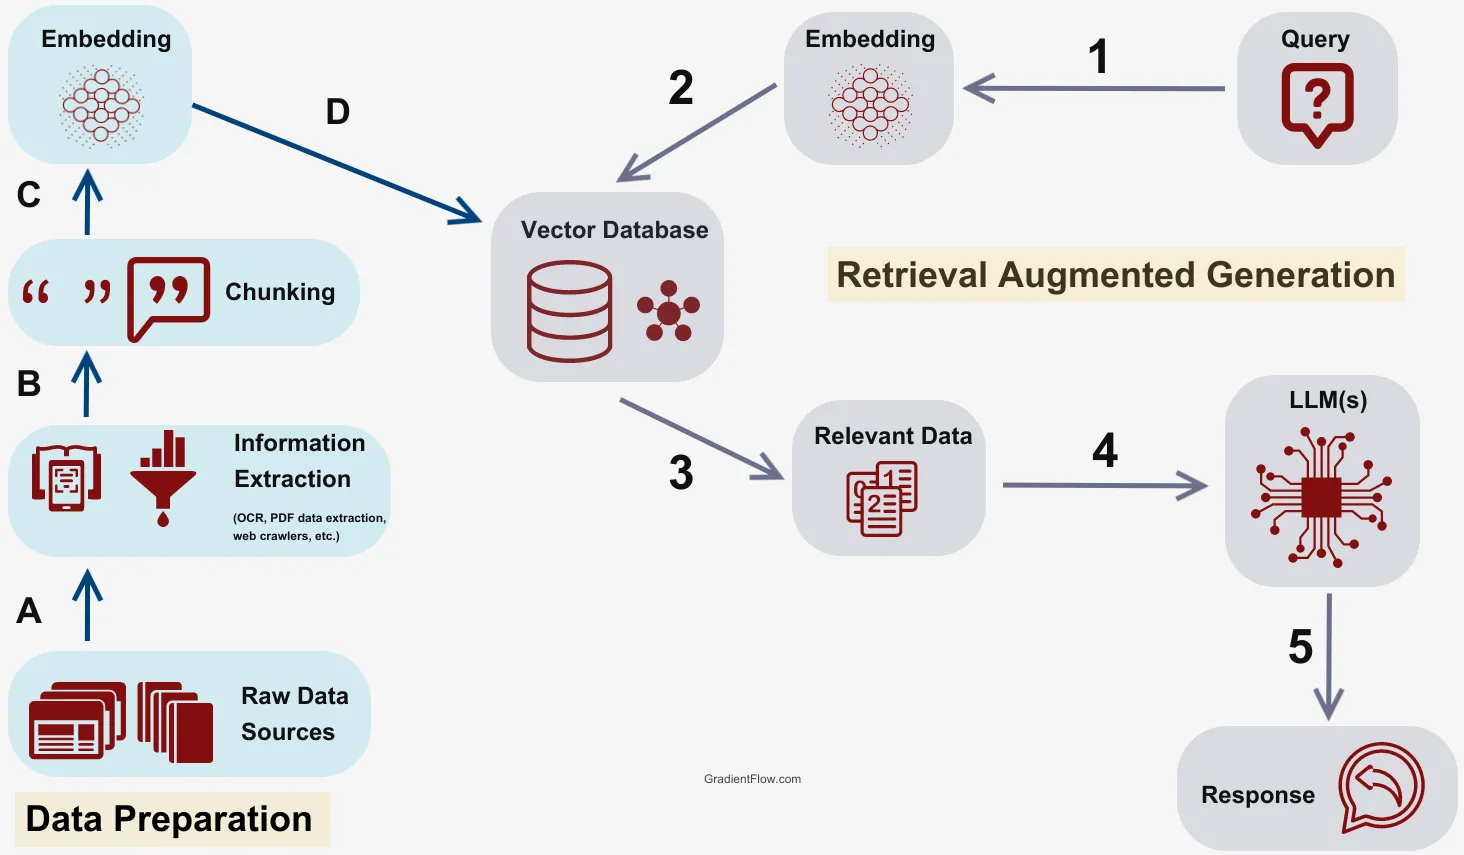
\includegraphics[width=\textwidth]{RAG.png}
		\centering
	\end{figure}
\end{displayquote}
\newpage

RAG kan hier dienst doen als een mogelijke plaatsvervanger voor manuele research en het opstellen van communicatiedocumenten (zoals aangetekende brieven, invorderingen, ...). Deze optie zal in
een later stadium van deze bachelorproef geëvealueerd worden. Advocatuur is een heel toepasselijk gebied voor RAG:

\begin{displayquote}
	Practically, RAG is likely preferable in environments like
	legal, customer service, and financial services where the ability to
	dynamically pull vast amounts of up-to-date data enables the most accurate and comprehensive responses.
\end{displayquote}



%%=============================================================================
%% Methodologie
%%=============================================================================

\chapter{\IfLanguageName{dutch}{Methodologie}{Methodology}}%
\label{ch:methodologie}

%% TODO: In dit hoofstuk geef je een korte toelichting over hoe je te werk bent
%% gegaan. Verdeel je onderzoek in grote fasen, en licht in elke fase toe wat
%% de doelstelling was, welke deliverables daar uit gekomen zijn, en welke
%% onderzoeksmethoden je daarbij toegepast hebt. Verantwoord waarom je
%% op deze manier te werk gegaan bent.
%% 
%% Voorbeelden van zulke fasen zijn: literatuurstudie, opstellen van een
%% requirements-analyse, opstellen long-list (bij vergelijkende studie),
%% selectie van geschikte tools (bij vergelijkende studie, "short-list"),
%% opzetten testopstelling/PoC, uitvoeren testen en verzamelen
%% van resultaten, analyse van resultaten, ...
%%
%% !!!!! LET OP !!!!!
%%
%% Het is uitdrukkelijk NIET de bedoeling dat je het grootste deel van de corpus
%% van je bachelorproef in dit hoofstuk verwerkt! Dit hoofdstuk is eerder een
%% kort overzicht van je plan van aanpak.
%%
%% Maak voor elke fase (behalve het literatuuronderzoek) een NIEUW HOOFDSTUK aan
%% en geef het een gepaste titel.

In dit hoofdstuk volgt wat er precies zal gebeuren om een RAG client app te bouwen die toepasbaar kan zijn voor grote datasets zoals die van Deltalex Advocaten. 
De volgende hoofdstukken zullen uitgebreid beschreven, onderzocht en uitgetest worden. \\

Het onderzoek naar oplossingen is parallel gevoerd samen met het opbouwen van een stappenplan om een werkende generieke digitale assistent te bekomen. 
Eerst worden de stappen van het onderzoek overlopen, dan gaan we naadloos over naar onderzoek over welke stappen en technologieën er aan bod komen in de ontwikkeling van een digitale assistent. 

\begin{enumerate}
    \item \textbf{Onderzoek: Requirements-analyse}
    \item \textbf{Onderzoek: Literatuurstudie}
    \item \textbf{Onderzoek: Haalbaarheid en dataveiligheid} 

    \item \textbf{Development: Documentdatabase}
    \item \textbf{Development: Context-aware chunking van verzamelde data}
    \item \textbf{Development: Integreren van Ollama met documentdatabase}
    \item \textbf{Development: Implementeren van een chatfrontend}
    \item \textbf{Development: Opzetten van lokale omgeving en componenten verbinden}
    \item \textbf{Development: Optimaliseren en testen}  

    \item \textbf{Resultaten}
\end{enumerate} 

%%Op het einde van deze reis is de uitkomst een digitale assistent die kennis heeft van alle dossierdata van een hypothetisch advocatenkantoor. 
%%Deze zal advocaten helpen met het opzoeken van informatie, opstellen van brieven, communicatie en dergelijke. 



\chapter{Technologieën}
\label{ch:technologies}
Alle technologieën hieronder besproken zijn allemaal vrij simpel vervangbaar in een modulair systeem zoals LangChain.

\section{Backend}
\subsection{Databases}
Een van de belangrijkste componenten van een chatbot die gebouwd is voor specifieke doeleinden, is een plaats om data te kunnen opslaan.
Een gesprek met een RAG app kan schematisch voorgesteld worden als volgt:

\begin{figure}[h]
	\makebox[\textwidth] {
		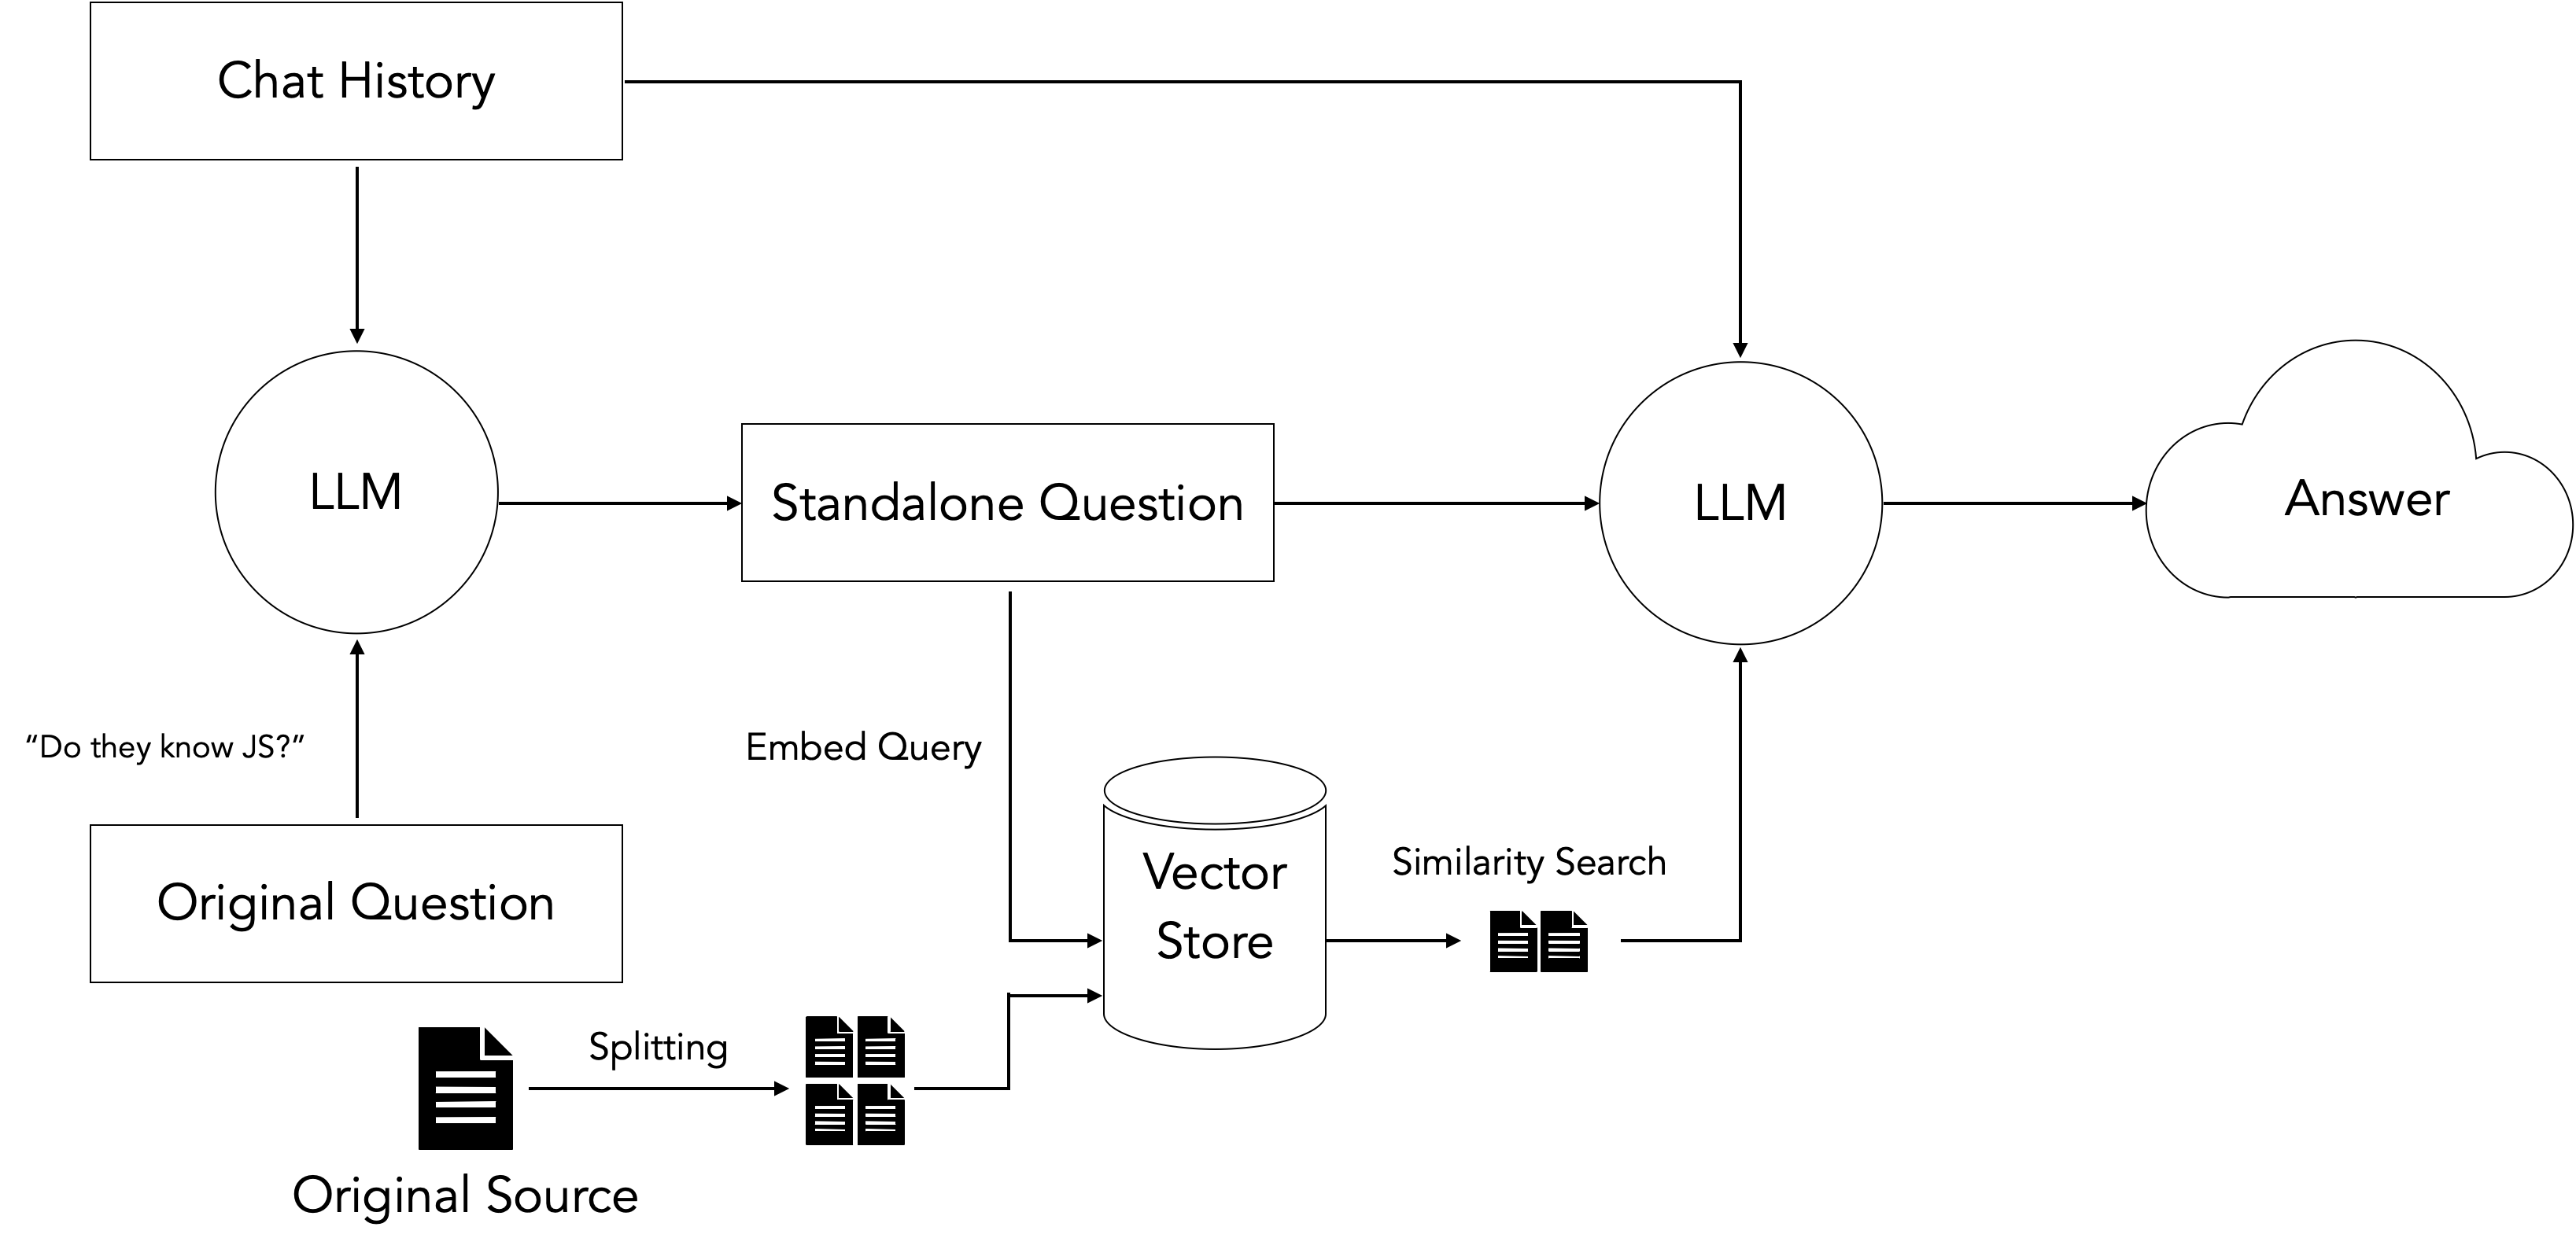
\includegraphics[width=\textwidth]{llm_pipeline.png}
	}
	\captionof{figure}{Schematische voorstelling van een conversatie met een LLM chatbot \autocite{Ollama} }
\end{figure}

Hier valt op dat een LLM niet alleen de vraag van de gebruiker in acht neemt, maar ook relevante documenten opvraagt uit een Vector store. 

\subsubsection{Vectorstore: Chroma}
De eerste keuze die moet worden gemaakt is welke vectorstore te gebruiken. Veel bronnen op het web bespreken open-source databases zoals Weaviate, Opensearch, Qdrant en \textbf{Chroma}. 
Chroma biedt ondersteuning met LangChain en kan gemakkelijk lokaal gedraaid worden. 
Chroma is de keuze die door LangChain aangeraden wordt als lokaal alternatief voor een online instantie van Weaviate.  
Omdat we met gevoelige documenten werken, willen we Deltalex Chat graag volledig lokaal houden dus vandaar zullen we voor Chroma kiezen als onze lokale vectorstore. 

\subsubsection{Record store: PostgreSQL}
Een vectorstore is een grote ongestructureerde ruimte met alle berekende vectoren en documentdata. 
Het kan handig zijn om naast deze ruimte een externe database bij te houden die bijvoorbeeld transactionele data (welke documenten er in de vectorstore zijn gegaan en wanneer), 
gebruikersdata en andere gestructureerde data bijhoudt. Dit is in ons proof-of-concept niet van gigantisch belang dus houden we het hier op een relatief simpele open-source database  
die voor veel developers de eerste keuze is: \textbf{PostgreSQL}. 

\subsection{Centraal verwerkingssysteem}
Om alles samen te gieten en te beheren, hebben we een modulair systeem nodig dat we ofwel volledig zelf kunnen bouwen, of kunnen overnemen van een open-source framework. 
Eén van de populairste én best gedocumenteerde frameworks hiervoor is \textbf{LangChain}. 
De missie van Langchain is om de volledige levenscyclus van AI systemen makkelijker te maken om te beheren. 
Zo kan men zijn eigen systeem schrijven met modulaire bouwblokken die allemaal open-source zijn en dit integreren met third-party clients zoals AWS, Google, OpenAI, ... \\ 

De keuze voor Deltalex Chat zal dan ook naar LangChain gaan omdat het heel flexibel is. 
Allerbelangrijkst is het ook volledig lokaal draaibaar en open-source. 

\newpage
\subsection{Modelkeuze en beheer}
Een van de belangrijkste componenten van een digitale assistent is vanzelfsprekend artificiële intelligentie. 
Er wordt op twee plaatsen in de toepassing gebruikt gemaakt van AI: 

\begin{itemize}
	\item Tijdens het genereren van embeddings
	\item Tijdens het chatten en genereren van documenten
\end{itemize}

Voor deze twee doelen hebben we twee verschillende modellen nodig. 
Omdat alles lokaal zal draaien, hebben we een toepassing nodig op ons systeem om modellen te draaien en te beheren. 
Een toepassing die de laatste tijd heel erg populair aan het worden is in de open-source AI wereld, is \textbf{Ollama}. 
Ollama is een programma dat toestaat als gebruiker (via command line) modellen lokaal te downloaden, beheren en te draaien. 
De modellen kunnen via een interactieve Python prompt gebruikt worden of via een exposed API. 
Dit maakt het mogelijk om (via een community plugin) aangesproken te worden door LangChain. 

\subsubsection{Embedding model}
Het is niet mogelijk om documenten rechtstreeks in een vectorstore te plaatsen. 
Er moeten eerst van die documenten stukken tekst(chunks) gemaakt worden. 
Op basis van die chunks moeten er vectoren berekend worden, waarop de vectorstore kan checken of een stuk tekst relevant is met de query van de gebruiker of niet. 
Om deze te berekenen, wordt er gebruik gemaakt van een text-embedding model. 
Dit zal de tekstuele informatie overzetten naar dergelijke vectoren die compatibel zijn met Chroma. \\

Er zijn veel embedding modellen beschikbaar via Ollama, waarvan het populairste \textbf{nomic-embed-text}. 
Nomic heeft tot nu toe al rond de 350 duizend downloads van Ollama en is dus veruit het meest gedownloade. 
De keuze hiervoor is dan ook snel gemaakt. 

\subsubsection{Large language model}
Large Language Models zijn de laatste tijd gigantisch populair geworden door bv. ChatGPT van OpenAI.
Hun bijna menselijke interactie zorgt ervoor dat een gebruiker de indruk heeft dat hij aan het praten is met een menselijke assistent maar dan veel sneller en 'slimmer'.\\

Natuurlijk is niets minder waar.
Een Large Language Model is immers een soort transformer, die de input (of query) van een gebruiker 'transformeert' naar een antwoord door de volgende token (woord) te voorspellen.
Deze modellen kunnen gegeneraliseerd worden voor verschillende use cases, niet zoals hun voorgangers zoals een PLM (Pretrained Language Model).
Het verschil hier is vooral de gigantische dataset waarop LLM's getrained worden.
Dit maakt ze toepasbaar op een veel breder gebied zonder enige extra configuratie of aanpassing.

Er zijn de laatste tijd heel veel modellen (zowel open- als closed-source) op de markt gekomen. Dit maakt het moeilijk om te kiezen voor een large-language-model voor onze implementatie. 
Volgens populariteit bij het ollama modelregister zijn llama3, Gemma, Qwen en \textbf{Mistral} de bekendste. De eerste drie zijn van Meta, Google en Alibaba. \\

In deze proof-of-concept zal Mistral gebruikt worden. Het is natuurlijk altijd mogelijk om te testen tussen verschillende modellen om te zien wat de advocaat in kwestie verkiest. 

\section{Frontend}
Het is natuurlijk niet echt aantrekkelijk voor een advocaat om alles te doen via command line, aangezien dit voor hun niet echt intuïtief en gebruiksvriendelijk is. 
Daarom is het maken van een aantrekkelijke en gebruiksvriendelijke frontend een absolute must in onze POC. \\ 

Er zijn heel veel repositories online die al een vooraf geïmplementeerde chat-interface bevatten, die makkelijk via een NodeJS library kan gerund en getest worden. 
Deze oplossingen bieden een goede basis voor de ontwikkeling van een frontend, maar moeten aangepast worden om te conformeren aan de huisstijl van Deltalex en om te verzekeren dat ze alleen maar het absolute nodige weergeven. \\

De implementatie hier zal gebeuren met een NodeJS library genaamd \textbf{NextJS} en de communicatie zal verlopen via \textbf{FastAPI}.


In het volgende hoofdstuk zullen we verder ingaan op de implementatie van de frontend. 
We zullen met screenshots de werking verduidelijken en uitleggen. 

\chapter{Implementatie}
\label{ch:implementation}
Dan is het nu tijd om onze POC te implementeren met de technologieën die hierboven besproken zijn.
Hieronder wordt gepoogd om zo specifiek mogelijk uit te leggen wat de verschillende ontwikkelingsstappen zijn en wat de manier is waarop deze zijn geïmplementeerd.

Dit project is geforked van chat-langchain, een voorbeeldimplementatie gebruikt door langchain om te chatten met hun developerdocumentatie.
Langchain host dit normaliter in de cloud, dus is er wat aanpassingswerk nodig om ervoor te zorgen dat alles veilig lokaal draait in een gecontroleerde omgeving.

\section{Writeup: Backend}
Deze sectie handelt over het instellen van het LangChain en Ollama systeem en het in staat te stellen om met FastAPI te communiceren met onze NextJS frontend.

\subsection{Geïnstalleerde software}
Vooraleerst hebben we een selectie aan software nodig om alles lokaal te kunnen draaien:
\begin{itemize}
	\item \textbf{Docker + compose plugin}
	\item \textbf{Python3 + pipx + poetry venv manager}
	\item \textbf{Ollama}
	\item \textbf{Embeddings model: nomic-embed-text}
	\item \textbf{Large-language-model: mistral}
	\item \textbf{Chroma}
	\item \textbf{PostgreSQL}
\end{itemize}

Chroma kan gecloned worden via \url{git@github.com:chroma-core/chroma.git} en gerund worden via \lstinline{docker compose up -d --build} in de geclonede directory. \\
Postgres kan gepulled worden van docker hub via \lstinline{docker pull postgres} en gerund worden via \lstinline{docker run -d --name postgres -e POSTGRES\_PASSWORD=root postgres} . \\

Als alles goed draait en als je een list command runt voor docker zal er een gelijkaardige output verschijnen zoals onderstaande screenshot:
\begin{figure}[h]
	\makebox[\textwidth]{
		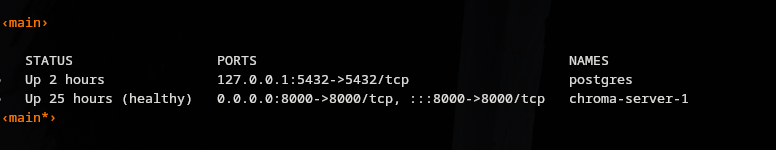
\includegraphics[width=\textwidth]{docker_containers.png}
	}
\end{figure}

Ollama kan geïnstalleerd worden via hun site \url{https://ollama.com} en dan via een command prompt kan je de modellen downloaden: \lstinline{ollama pull nomic-embed-text \&\& ollama pull mistral}. \\

Alle andere packages zijn normaal beschikbaar uit de package repositories van alle populaire distributies.

\subsection{Opzetten van lokale omgeving}
Allereerst zullen we het project importeren dat we zullen aanpassen, dit kan gecloned worden via \lstinline{git clone --branch langserve --single-branch https://github.com/langchain-ai/chat-langchain/}.
Daarna installeren we alle packages in onze repository via \lstinline{poetry install}. Dit creëert een virtuele python omgeving. Installeer ook de pypdf module via \lstinline{poetry add pypdf}.
Virtuele python omgevingen zijn handig als je geen dependency hell wilt veroorzaken met meerdere projecten op dezelfde machine. \\

Nu hebben we nog documenten nodig.
Er zijn een aantal documenten van Deltalex verkregen en samen met een paar publieke wetboeken (om de schrijfstijl en het vocabularium van een advocaat na te bootsen) geplaatst in een directory.
Deze documenten verschillen van brieven, mails tot ingebrekestellingen en worden puur ter referentie gebruikt.

\subsection{Instellen van vectorstore en record store - ingest script}
Nu we alles hebben opgezet is het nog nodig om ons ingest script wat aan te passen om puur lokaal te draaien. Hierna volgt de implementatie gebruikt voor ons POC:
\newpage

\begin{lstlisting}
import logging
import os

from chromadb import HttpClient
from chromadb.config import Settings
from langchain.text_splitter import RecursiveCharacterTextSplitter
from langchain_core.embeddings import Embeddings
from langchain_chroma import Chroma
from langchain.indexes import SQLRecordManager, index
from langchain_community.embeddings.ollama import OllamaEmbeddings
from langchain_community.document_loaders import PyPDFDirectoryLoader
# add pypdf module to venv


logging.basicConfig(level=logging.INFO)
logger = logging.getLogger(__name__)


def get_embeddings_model() -> Embeddings:
    return OllamaEmbeddings(model="nomic-embed-text:latest")


def load_deltalex_pdfset():
    return PyPDFDirectoryLoader("/home/laurent/Documents/schoolrepos/HoGent1/bachelorsAssignment/deltalexDocs/").load()


def getChromaClient():
    return HttpClient(settings=Settings(anonymized_telemetry=False))


def ingest_docs():
    DATABASE_HOST = os.environ["DATABASE_HOST"]
    DATABASE_PORT = os.environ["DATABASE_PORT"]
    DATABASE_USERNAME = os.environ["DATABASE_USERNAME"]
    DATABASE_PASSWORD = os.environ["DATABASE_PASSWORD"]
    DATABASE_NAME = os.environ["DATABASE_NAME"]
    RECORD_MANAGER_DB_URL = f"postgresql://{DATABASE_USERNAME}:{DATABASE_PASSWORD}@{DATABASE_HOST}:{DATABASE_PORT}/{DATABASE_NAME}"
    COLLECTION_NAME = os.environ["COLLECTION_NAME"]

    vectorstore = Chroma(
        collection_name=COLLECTION_NAME,
        embedding_function=get_embeddings_model(),
        persist_directory="./deltalex_chroma",
        client=getChromaClient()
    )

    text_splitter = RecursiveCharacterTextSplitter(chunk_size=224, chunk_overlap=32)

    record_manager = SQLRecordManager(
        namespace="deltalex",
        db_url=RECORD_MANAGER_DB_URL
    )
    record_manager.create_schema()

    docs_transformed = text_splitter.split_documents(load_deltalex_pdfset())
    logger.info("docs transformed")

    indexing_stats = index(
        docs_transformed,
        record_manager,
        vectorstore,
        cleanup="full",
        source_id_key="source"
    )

    logger.info(indexing_stats)
    logger.info("docs added to vector database")


if __name__ == "__main__":
    ingest_docs()

\end{lstlisting}
Deze implementatie heeft een groot aantal verschillen van de originele github code. Allereerst worden er documenten uitgelezen uit een specifieke map naar mijn keuze.
Vervolgens worden ze gesplit in chunks tekst (van in totaal 256 karakters en wat overloop ingerekend) om dan doorgestuurd te worden naar een lokale Ollama instantie,
die ze transformeert naar vectoren in toevoegt in de database. \\

De volledige implementatie is lokaal en zal het netwerk van de machine niet verlaten.
De connectiestrings voor PostgreSQL worden uitgelezen uit environment variables.
De parameters voor een default chroma \lstinline{HttpClient} komen overeen met de settings van een docker compose container.
Een extra parameter voor anonymized telemetry zorgt ervoor dat er geen anonieme statistieken naar Chroma verstuurd worden. \\

Hier wordt ook voor het \lstinline{nomic-embed-text} model gekozen via OllamaEmbeddings.
Dat is een voorbeeld van een third party plugin van LangChain.

Het is de bedoeling dat dit script als eerst wordt gerund. Zonder vector store zal Deltalex Chat ook werken, maar zal er weinig relevante info gegeven worden door mistral alleen.
Als dit allemaal gerund heeft, is onze vectorstore klaar voor RAG gebruik.

\newpage
\subsection{Instellen van LLM en centraal systeem - Configureren van Langchain backend chain script}
\subsubsection{Aanpassing retriever}

Nu is het tijd om het systeem zelf te configureren. Veel van dit werk is al geïmplementeerd dankzij LangChain en de repo waarvan we gecloned hebben.
Deze klasse zorgt voor de interne afhandeling van requests aan ons systeem en is dus van elementair belang. \\ 

Dit systeem komt met een API voor later met onze frontend te communiceren en ook met een playground om prompts te testen en te zien wat er gebeurt achter de schermen. 
Het is eigenlijk de bedoeling om LangChain in de cloud te deployen (omdat cloud computers veelal sterkere grafische kaarten hebben en dus betere resultaten leveren)
maar via de tweaks die we nu maken is het mogelijk dit systeem volledig lokaal te draaien.\\

Allereerst passen we de vectorstore client weer aan naar Chroma en returnen we deze als vector retriever.
Deze functie zal dus verantwoordelijk zijn om relevante vectoren te retrieven en te gebruiken als context in het antwoord van onze LLM.
Dit is de functie in kwestie:

\begin{lstlisting}
def getChromaClient():
    return HttpClient(settings=Settings(anonymized_telemetry=False))


def get_retriever() -> BaseRetriever:
    vectorstore = Chroma(
        collection_name="deltalex",
        embedding_function=OllamaEmbeddings(model="nomic-embed-text:latest"),
        persist_directory="./deltalex_chroma",
        client=getChromaClient()
    )
    return vectorstore.as_retriever(search_kwargs=dict(k=6))

\end{lstlisting}

\newpage
\subsubsection{Prompt template}
Nu onze retriever is aangepast, is het ook heel belangrijk om een passend prompt template te maken voor onze Deltalex Chat.
Prompt templates zijn de wrapper rond LLM's. Een large language model heeft meestal een heel specifieke set instructies nodig om
naar behoren te functioneren. Deze prompt templates zijn ook wat een model de menselijke touch geeft.
Een voorbeeld van het gebruikte prompt template voor Deltalex Chat:

\begin{lstlisting}
    You are a lawyer, specialized in drafting legal documents for a Belgian law firm.
    From here on you write in Dutch. 
    This text from the context html tags is for linguistic purposes and to mimic a legal writing style. 
    
    Write a legal document, based on the provided context. 
    Use a professional and formal tone, suitable for a legal context. 
    
    Your writing style must be very formal and legal.
    Write in correct Dutch sentences and base yourself on the given documents inside the context html tags. 
    
    Anything between the following `context`  html blocks is retrieved from a set of legal documents.
    Use it as a linguistic reference. 
    You need to mimic the writing style to resemble that of a legal professional.
    
    <context> 
        {context}
    <context/>
    
    REMEMBER: 
    Do not write repetitive sentences. 
    Write in Dutch or French, based on the parameter given. Default will be Dutch. 
    Be very formal. 
\end{lstlisting}

De effectiviteit van een chatbot valt en staat met het prompt template. 
Het is niet simpel om een perfect template te fabriceren, maar gelukkig zijn er veel resources zoals \url{https://github.com/promptslab/Awesome-Prompt-Engineering?tab=readme-ov-file}
om ons daarmee te assisteren. \\

Dit is de laatste stap in het configuratieproces van het backend deel van onze implementatie. 

\newpage
\section{Frontend}
Deze sectie zal gaan over het aanpassen van de meegeleverde chat frontend naar onze wensen. 
Deze implementatie omvat een NextJS React project, gebouwd met ChakraUI en TailwindCSS. 

\subsection{Geïnstalleerde software}
Eerst installeren we best de software die we gaan gebruiken om het project te compileren. 
Dit korte lijstje omvat:

\begin{itemize}
    \item Node
    \item Een node package manager zoals npm, pnpm, yarn, ... 
\end{itemize}

Deze tools zijn makkelijk te installeren uit de package managers van iedere populaire distributie. 

\subsection{Aanpassing van waarden}
Er zijn veel waarden aangepast in de source files om de frontend zo minimaal en gebruiksvriendelijk mogelijk te maken. 
Dit bestand toont de volledige diff chart: \url{https://gist.github.com/DuquesnoyLaurent/f73ee763db497a3a2af6ecbc6d853f44}

Onderstaande screenshot geeft de frontend weer:
\begin{figure}[h]
    \makebox[\textwidth]{
	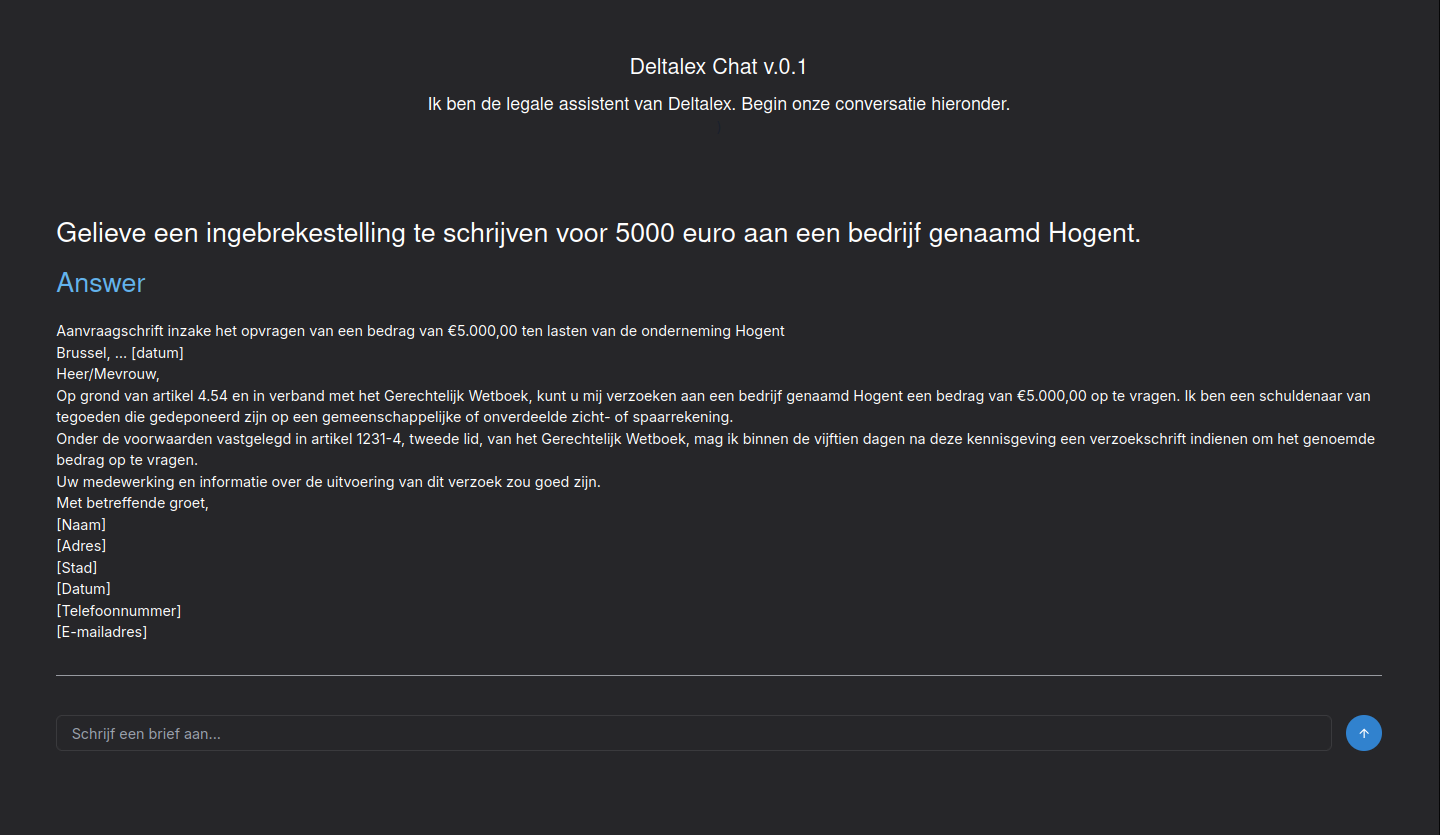
\includegraphics[width=\textwidth]{frontend.png}
    }
\end{figure}


\chapter{Resultaten en reflectie}
\label{ch:results_reflection}
Een reflectie verloopt heel goed aan de hand van auto-evaluatie d.m.v. vragen die men aan zichzelf stelt. 
Hieronder volgen een paar vragen die kunnen ontspringen wanneer men denkt aan automatisatie van workflows en repetitieve taken.\\ 

\textbf{Welke taken zijn er nu makkelijk te automatiseren?}
De taken die hier in deze bachelorproef beschreven worden gaan over:
\begin{itemize}
	\item \textbf{Opzoekingswerk verrichten in documentendatabases}
	\item \textbf{Opzoekingswerk verrichten in publieke databases}
	\item \textbf{Opstellen van documenten}
\end{itemize}
Een digitale assistent kan een advocaat helpen met deze taken te versnellen door tekst te genereren ter inspiratie en met relevante informatie uit een database. 
Het opstellen en gebruiken(versturen, indienen bij de rechtbank, ...) van deze documenten moet nog altijd gebeuren door de advocaat zelf. 
Een digitale assistent dient niet ter vervanging van een advocaat, maar wel als een tool die hun workflow kan versnellen. \\ 

\textbf{Hoeveel productiviteitswinst kan een advocaat realiseren bij deze taken?}
Het gebruik van een digitale assistent zal opzoekingswerk versnellen en dienen ter inspiratie. 
Om nog efficiënter te kunnen werken kan een advocaat technieken leren zoals sneltoetsen en tools gebruiken zoals browserextensies om hun workflow exponentieel te optimaliseren. 
Hoeveel productiviteitswinst er dan is, hangt af van advocaat tot advocaat. 
Sommigen zullen hun workflow bewaren zoals hij is en zijn er tevreden mee. 
Anderen zullen altijd op zoek zijn om deze te versnellen en te optimaliseren en kunnen zich hier ook actief mee bezighouden. 
Indien men de tijd wil vrijmaken om hier onderzoek naar te verrichten, zal er over de tijd een gestage stijging 
zijn in de snelheid van hun workflow door het gebruik van technieken en digitale assistenten. \\ 

\textbf{Waarmee moet men rekening houden bij de ontwikkeling van een digitale assistent?}
Het belangrijkste aspect bij de ontwikkeling van een digitale assistent bij een advocatenkantoor is waarschijnlijk dataveiligheid. 
Er mag absoluut, in geen enkele instantie twijfel ontstaan bij de gebruiker of bij de cliënt dat er vertrouwelijke data op het spel staat.  
Een dergelijk voorval zou potentieel destructief zijn voor de klantenrelaties en het imago van het advocatenkantoor. 
Andere belangrijke aspecten zijn gebruikersvriendelijkheid, snelheid van tokengeneratie en de kwaliteit van de gegenereerde antwoorden.\\ 

\textbf{Wat zijn de voor- en nadelen van een automatie via chatbots?}
De voordelen van chatbots zijn de snelheid van antwoorden, de bijna menselijke manier van interactie en de bron van inspiratie voor het opstellen van documenten. 
Chatbots zoals ChatGPT zijn de laatste jaren aan een gigantische opmars bezig en hun functionaliteiten worden alleen maar beter dankzij de gigantisch hoge graad van evolutie in de technologische sector. 
Nadelen van chatbots kunnen dingen zijn zoals hallucinatie(generatie van incorrecte antwoorden), grammaticale repetitie, ... 
Het is altijd aangeraden om hun output te valideren i.p.v. er blind op te vertrouwen. 

%%=============================================================================
%% Conclusie
%%=============================================================================

\chapter{Conclusie}%
\label{ch:conclusie}

% TODO: Trek een duidelijke conclusie, in de vorm van een antwoord op de
% onderzoeksvra(a)g(en). Wat was jouw bijdrage aan het onderzoeksdomein en
% hoe biedt dit meerwaarde aan het vakgebied/doelgroep? 
% Reflecteer kritisch over het resultaat. In Engelse teksten wordt deze sectie
% ``Discussion'' genoemd. Had je deze uitkomst verwacht? Zijn er zaken die nog
% niet duidelijk zijn?
% Heeft het onderzoek geleid tot nieuwe vragen die uitnodigen tot verder 
%onderzoek?

De uitkomst van dit onderzoek is een roadmap die informatie bevat over iedere component van de opbouw van een digitale assistent. 
Eerst was de opzet van dit onderzoek om een assistent te implementeren en te integreren met bestaande software. 

Natuurlijk werkt deze assistent met libraries en componenten die toch heel wat resources gebruiken om vloeiend te bouwen, draaien en testen. 
Dit in combinatie met de gevoeligheid van de cliëntdata is de beslissing gekomen om dit onderzoek puur hypothetisch uit te voeren. 
Denk over dit onderzoek als een stappenplan om een lezer bekend te maken met de basisconcepten van Natural Language Processing, Large Language Models, Retrieval Augmented Generation en meer. 

Veel stappen uit dit onderzoek worden minder breed besproken gezien het hedendaagse aanbod van digitale tools zoals JavaScript libraries, 
frameworks die al heel goeie implementaties voor digitale assistenten leveren en de extraordinaire snelle aard van verandering van het huidig technologisch spectrum. 

Er is in dit onderzoek geprobeerd om zo veel mogelijk technologiespecifiek te werken. 
Het kan goed zijn dat er binnenkort betere technologieën uitgebracht worden die veel beter presteren dan degene die hier gebruikt worden. 
De technologieën gebruikt in dit onderzoek zijn op het moment van onderzoek de meest geschikte en performante op de markt, waarvan de meeste open-source. 

In conclusie hoop ik dat een lezer van dit onderzoek enerzijds bijleert over digitale assistenten en hoe ze werken onder de motorkap. 
Anderzijds dat hij het ook kan gebruiken als stappenplan tijdens het implementeren van zijn eigen assistent, iets waar de student die er nu aan werkt ook zeker gebruik van zal maken. 


% Voeg hier je eigen hoofdstukken toe die de ``corpus'' van je bachelorproef
% vormen. De structuur en titels hangen af van je eigen onderzoek. Je kan bv.
% elke fase in je onderzoek in een apart hoofdstuk bespreken.


%---------- Bijlagen -----------------------------------------------------------

\appendix

\chapter{Onderzoeksvoorstel}

Het onderwerp van deze bachelorproef is gebaseerd op een onderzoeksvoorstel dat vooraf werd beoordeeld door de promotor. Dat voorstel is opgenomen in deze bijlage.

%% TODO: 
%\section*{Samenvatting}

% Kopieer en plak hier de samenvatting (abstract) van je onderzoeksvoorstel.

% Verwijzing naar het bestand met de inhoud van het onderzoeksvoorstel
%---------- Inleiding ---------------------------------------------------------
\section{Introductie}%
\label{sec:introductie}

Mijn bachelorproef spitst zich toe op het optimaliseren van de administratieve workload bij advocatenkantoor Deltalex. Dit zal gebeuren via het invoeren van geautomatiseerde processen, het
ontwikkelen van een centrale webinterface om opzoekwerk te verrichten, daarbij ook een portaal om de sjablonen van de meestgebruikte documenten bij te houden en te bewerken.

Dit onderzoek vindt zijn oorsprong in de vaststelling van veel tijdrovende en repetitieve taken die de efficiëntie van dit kantoor kunnen belemmeren,
zoals het handmatig opzoeken van cliëntgegevens in openbare databases en het bijwerken van veelgebruikte documenttemplates.

De onderzoeksvraag van mijn bachelorproef luidt: "Hoe kunnen geautomatiseerde processen, in combinatie met een webinterface voor beheer, de administratieve
last in advocatenkantoren verminderen en de efficiëntie bevorderen?"

Het beoogde eindresultaat omvat niet alleen een werkend prototype van automatisatie en de bijbehorende webinterface,
maar ook een grondig rapport met aanbevelingen voor implementatie in advocatenkantoren.

Het succes van deze bachelorproef zal worden beoordeeld aan de hand van daadwerkelijke verbeteringen in efficiëntie en
tijdsbesparing binnen advocatenkantoor Deltalex.

%---------- Stand van zaken ---------------------------------------------------
\section{Literatuurstudie: automatisatie en de selectie van CMS's in de advocatuur}%
\label{sec:state-of-the-art}

Consider one real-world example: if your firm had 12,000 documents to review, and each one had 75 questions to answer, the task will take weeks to complete. Even with a sizable team working in concert, the sheer volume of work is daunting. One of those, “Where do I even start?” types of tasks others might shrink from.
But what if you started by working the process, not just digging into the work? By automating even a part of a task that large, you stand to shave hours off the time involved.
\autocite{ThomsonReuters2023}

Deze citatie illustreert dat investeren in een efficiëntere aanpak van je repetitieve taken zeker kan lonen. Dit is natuurlijk ook toepasbaar op een advocatenkantoor, volgende citatie illustreert het maken van documenten, waaronder dagvaardingen, invorderingen en mails.

Document creation, for example, requires a large amount of repetitive work. Diving right into the work may seem like the best way to get ahead, but by taking the time to define the fields in a document, and set up corresponding variables, it’s easy for a computer to automatically create custom, accurate documents on a scale that no human can match.
\autocite{ThomsonReuters2023}

Automatisatie kan ook executie van taken zoals indienprocedures en legal research exponentieel sneller maken. \autocite{Aston2023}

Het huidige landschap van administratieve\\ tools is heel groot. In het geval van Deltalex (en andere kantoren) hebben ze gekozen voor een bepaald softwarepakket. Dit is veelal een moeilijke keuze omdat er heel veel pakketten beschikbaar zijn en deze bieden elk hun voor- en nadelen. De selectie van een dergelijke tool kan een moeizaam proces zijn, maar kan gegoten worden in volgende stappen.
\autocite{Clio2023}

\begin{itemize}
	\item \emph{Kies tussen cloud- of lokale opslag:} Waar hosten? 
        \item \emph{Bekijk de kosten- en onderhoudsverschillen:} Varieert sterk op basis van stap 1.
        \item \emph{Zorg voor toegang tot informatie op afstand:} Veel advocaten werken soms op afstand, bv. vanuit een rechtbank.
        \item \emph{Controleer de compatibiliteit met bestaande software:}\\ Complexere pakketten worden meestal pas aangekocht als het kantoor zich verder bevindt dan de startfase. M.a.w. er is zeker al bestaande data op oudere systemen.
        \item \emph{Evalueer gebruiksgemak en trainingsvereisten:} Het is belangrijk dat iedere gebruiker zo snel en probleemloos met de nieuwe software aan de slag kan.
        \item \emph{Zorg voor ethische naleving en beveiliging:} Advocatenkantoren werken onder strikte regels voor professioneel gedrag, daarom is het aangeraden om voor gespecialiseerde software te opteren.
\end{itemize}

Dergelijke pocessen kunnen lang duren en in het geval van Deltalex is dit al gebeurd. Daarom bespreek ik in deze bachelorproef de ontwikkeling van een externe interface om specifieke taken sneller af te handelen.

%---------- Methodologie ------------------------------------------------------
\section{Methodologie}%
\label{sec:methodologie}
Deze bachelorproef zal een combinatie zijn van een case study in advocatenkantoor Deltalex en een proof of concept van het platform om in het kantoor de administratieve workload zoveel mogelijk te minimaliseren. Deze implementatie valideert de haalbaarheid en de effectiviteit van de oplossing doorheen heel het kantoor, beginnende bij één specifieke advocaat. 

Het onderzoek zal zich concentreren op accurate en objectieve resultaten en vermijdt onderzoekstechnieken die subjectieve data yielden, zoals enquêtes. Literatuurstudie, interviews en praktische data zullen de bouwstenen zijn van het uiteindelijke verdict van de implementatie. 

De voorgaande technische analyse zal voor mij een unieke kans zijn om op zowel het informaticadomein als in de administratieve/ juridische sector mijn skills bij te scherpen. Er zullen tools gebruikt worden als front-end-webassembly talen voor een moderne approach van een webinterface. Voor automatisatie van queries online zal er gebruik gemaakt worden van scripttalen en er zal ook grondig uitgezocht worden hoe men sjablonen zo effectief mogelijk kan aanpassen via MS Office XML-injecties in documenten. 

Deze proef zal 12 weken in beslag nemen en is optimaal zoals onderstaand ingedeeld:
\begin{itemize}
        \item Requirementanalyse: 2 weken.\\ \emph{Deliverable} -> Verslag van requirements
        \item Ontwerp en technologieselectie: 2 weken.\\ \emph{Deliverable} -> technologiestack en praktische planning voor implementatie
        \item Implementatie: 4 weken.\\ \emph{Deliverable} -> werkende proof of concept
        \item Evaluatie: 2 weken. \\ \emph{Deliverable} -> Evaluatierapport
        \item Aanpassen van project en conclusie: 2 weken.\\ \emph{Deliverable} -> Aangepaste proof of concept, eindrapport en conclusie
\end{itemize}

%---------- Verwachte resultaten ----------------------------------------------
\section{Verwacht resultaat, conclusie}%
\label{sec:verwachte_resultaten}
Ik verwacht natuurlijk dat Deltalex geniet van mijn oplossing en dat alle vennoten hun tijd kunnen investeren in dingen die écht belangrijk zijn. Daarmee vermijden ze repetitieve taken die heel tijdrovend zijn. Ook zal de stress en frustratie op de werkvloer afnemen. Dat zal resulteren in een aangename werkomgeving waar iedereen zich productief bezighoudt en zichzelf amuseert in hun werk.

Naar de praktische kant toe verwacht ik drie dingen:
\begin{itemize}
        \item \emph{Requirementsanalyse}
        \item \emph{Ontwerp en implementatie van gekozen technologieën}
        \item \emph{Evaluatie en validatie}
\end{itemize}

Ik hoop ook dat mijn bachelorproef kan motiveren waarom een kantoor (in dit geval advocatenkantoor) voordeel zou kunnen halen uit specifieke implementaties, die kunnen helpen aan bepaalde nicheproblemen, zonder een volledig nieuw systeem te implementeren. Een nieuw systeem moet aangekocht, aangeleerd en aangepast worden. Dit is een kwestie van hoge kosten, potentieel lange gewenning en mogelijke datamigratieproblemen. 


%%---------- Andere bijlagen --------------------------------------------------
% TODO: Voeg hier eventuele andere bijlagen toe. Bv. als je deze BP voor de
% tweede keer indient, een overzicht van de verbeteringen t.o.v. het origineel.
%\input{...}

%%---------- Backmatter, referentielijst ---------------------------------------

\backmatter{}

\setlength\bibitemsep{2pt} %% Add Some space between the bibliograpy entries
\printbibliography[heading=bibintoc]

\end{document}
